\documentclass[12pt]{letter}\usepackage[letterpaper,margin=0.65in]{geometry}\usepackage{textcomp}\usepackage{graphicx}\usepackage[rflt]{floatflt}\pagenumbering{gobble}\begin{document}\begin{floatingfigure}{0.15\textwidth}\raisebox{0pt}[0pt][0pt]{\raisebox{-2.5cm}{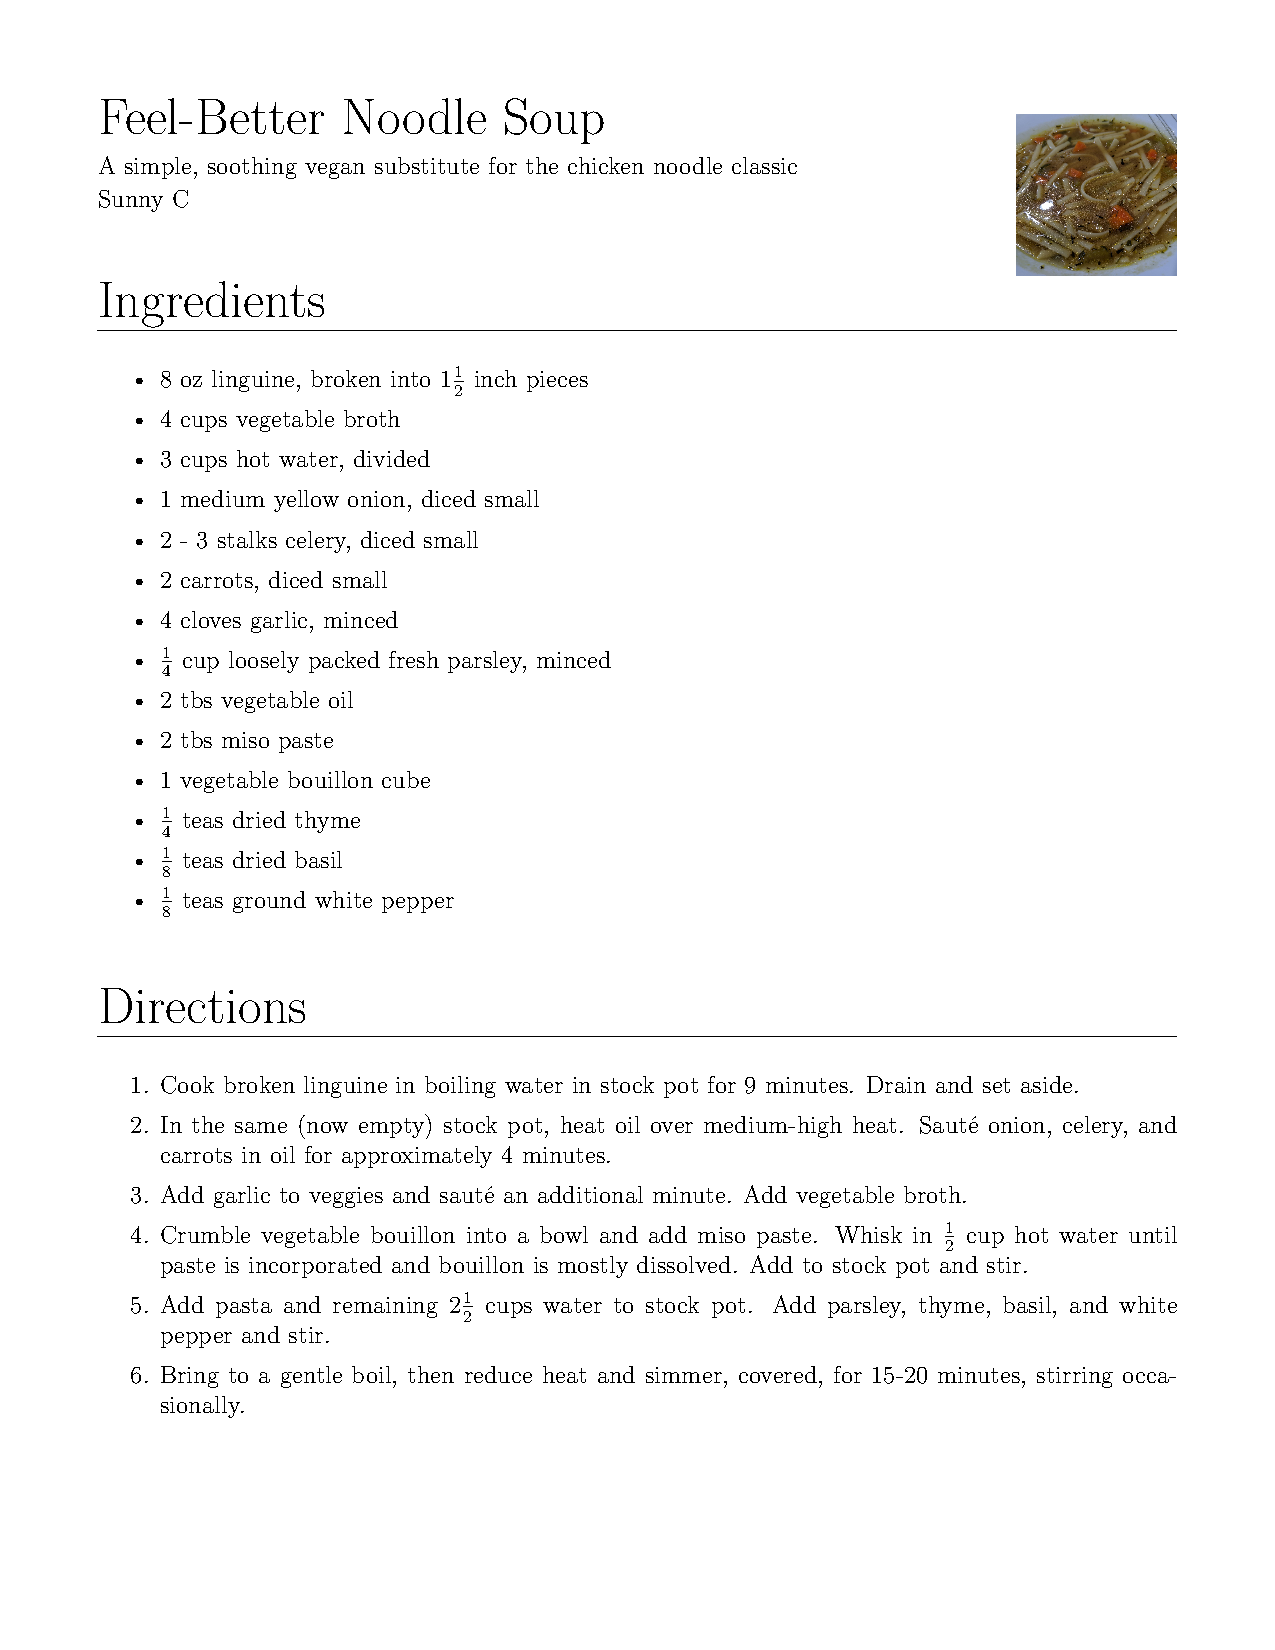
\includegraphics[width=0.15\textwidth]{feel-better-noodle-soup}}}\end{floatingfigure}\begin{huge}Feel-Better Noodle Soup\end{huge}\newline\vspace{-2.5mm}\newline\renewcommand{\arraystretch}{1.1}\begin{tabular*}{\textwidth}{@{\extracolsep{\fill}}lr}A simple, soothing vegan substitute for the chicken noodle classic\\Sunny C\end{tabular*}\newline\vspace{10mm}\newline\begin{huge}Ingredients\end{huge}\\\rule[2.8mm]{\textwidth}{.1pt}\vspace{-3mm}\begin{itemize}\item 8 oz linguine, broken into 1$\frac{1}{2}$ inch pieces\item 4 cups vegetable broth\item 3 cups hot water, divided\item 1 medium yellow onion, diced small\item 2 - 3 stalks celery, diced small\item 2 carrots, diced small\item 4 cloves garlic, minced\item $\frac{1}{4}$ cup loosely packed fresh parsley, minced\item 2 tbs vegetable oil\item 2 tbs miso paste\item 1 vegetable bouillon cube\item $\frac{1}{4}$ teas dried thyme\item $\frac{1}{8}$ teas dried basil\item $\frac{1}{8}$ teas ground white pepper\end{itemize}\vspace{7mm}\begin{huge}Directions\end{huge}\\\rule[2.8mm]{\textwidth}{.1pt}\vspace{-3mm}\begin{enumerate}\item Cook broken linguine in boiling water in stock pot for 9 minutes. Drain and set aside.\item In the same (now empty) stock pot, heat oil over medium-high heat. Sauté onion, celery, and carrots in oil for approximately 4 minutes.\item Add garlic to veggies and sauté an additional minute. Add vegetable broth.\item Crumble vegetable bouillon into a bowl and add miso paste. Whisk in $\frac{1}{2}$ cup hot water until paste is incorporated and bouillon is mostly dissolved. Add to stock pot and stir.\item Add pasta and remaining 2$\frac{1}{2}$ cups water to stock pot. Add parsley, thyme, basil, and white pepper and stir.\item Bring to a gentle boil, then reduce heat and simmer, covered, for 15-20 minutes, stirring occasionally.\end{enumerate}\end{document}